\begin{minipage}{0.49\textwidth}
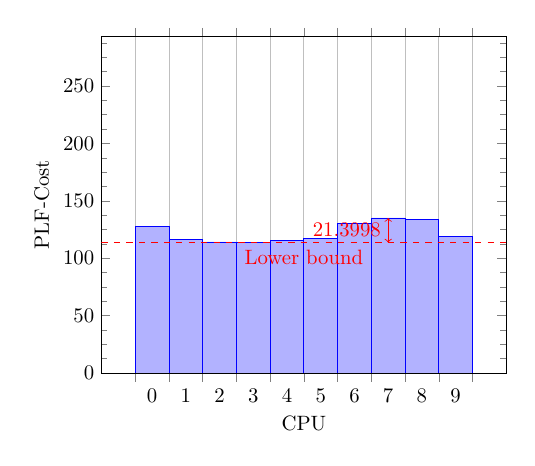
\begin{tikzpicture}[scale=0.75]
  \begin{axis}[ybar interval, ymax=292.908,ymin=0, minor y tick num = 3
, xlabel={CPU}, ylabel={PLF-Cost}]
    \addplot coordinates { (0,127.474) (1,116.335) (2,114.154) (3,113.707) (4,115.744) (5,117.437) (6,130.194) (7,135.012) (8,134.012) (9,118.663) (10, 133.14) };
\draw [red, dashed] ({rel axis cs:0,0}|-{axis cs:0,113.613}) -- ({rel axis cs:1,0}|-{axis cs:10,113.613}) node [pos=0.5, below] {Lower bound};
\draw [red, <->] ({axis cs:7.5,113.613}) -- ({axis cs:7.5,135.012}) node [pos=0.5, left] { 21.3998};
  \end{axis}
\end{tikzpicture}
\caption*{Weights repartition on the first tree}
\end{minipage}
\begin{minipage}{0.49\textwidth}
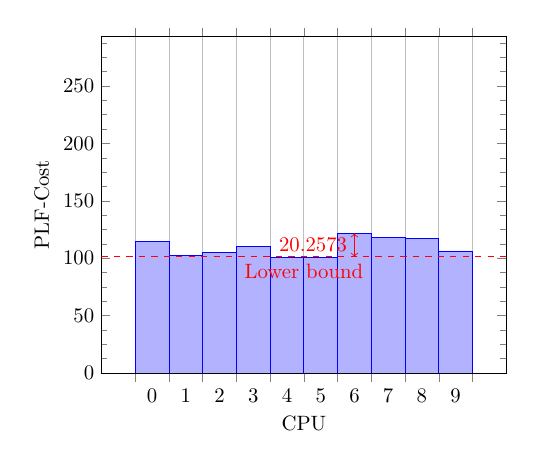
\begin{tikzpicture}[scale=0.75]
  \begin{axis}[ybar interval, ymax=292.908,ymin=0, minor y tick num = 3
, xlabel={CPU}, ylabel={PLF-Cost}]
    \addplot coordinates { (0,114.476) (1,102.439) (2,104.985) (3,109.96) (4,100.28) (5,100.831) (6,121.561) (7,117.886) (8,117.471) (9,106.305) (10, 133.14) };
\draw [red, dashed] ({rel axis cs:0,0}|-{axis cs:0,101.303}) -- ({rel axis cs:1,0}|-{axis cs:10,101.303}) node [pos=0.5, below] {Lower bound};
\draw [red, <->] ({axis cs:6.5,101.303}) -- ({axis cs:6.5,121.561}) node [pos=0.5, left] { 20.2573};
  \end{axis}
\end{tikzpicture}
\caption*{Weights repartition on the last tree}
\end{minipage}
\begin{minipage}{0.49\textwidth}
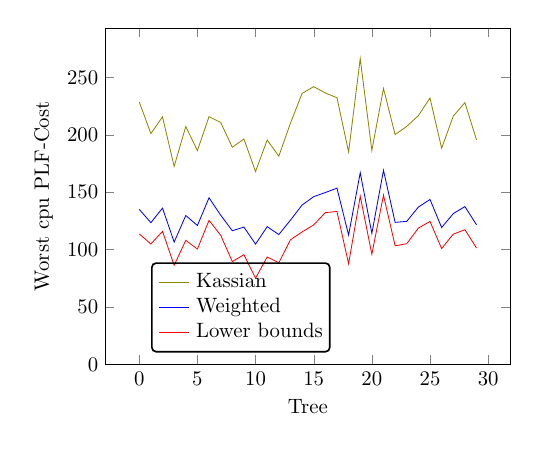
\begin{tikzpicture}[scale=0.75]
  \begin{axis}[ymax=292.908,ymin=0
, xlabel={Tree}, ylabel={Worst cpu PLF-Cost}]
    \addplot[mark=., color=blue] coordinates { (0,135.012) (1,123.397) (2,136.077) (3,106.474) (4,129.623) (5,120.935) (6,145.097) (7,129.968) (8,116.39) (9,119.531) (10,104.734) (11,119.906) (12,113.035) (13,125.608) (14,138.757) (15,146.067) (16,149.655) (17,153.474) (18,112.6) (19,166.921) (20,114.082) (21,169.032) (22,123.67) (23,124.558) (24,136.988) (25,143.635) (26,119.171) (27,131.293) (28,137.372) (29,121.561) };
    \addplot[mark=., color=olive] coordinates { (0,228.591) (1,200.998) (2,215.598) (3,172.402) (4,207.124) (5,186.233) (6,215.734) (7,210.712) (8,189.084) (9,196.313) (10,167.935) (11,195.432) (12,181.295) (13,210.084) (14,235.978) (15,241.883) (16,236.367) (17,232.231) (18,185.005) (19,266.28) (20,186.335) (21,240.323) (22,200.122) (23,207.315) (24,216.64) (25,232) (26,188.211) (27,216.189) (28,227.995) (29,195.548) };
    \addplot[mark=., color=red] coordinates { (0,113.613) (1,104.86) (2,115.85) (3,86.2638) (4,107.974) (5,100.396) (6,125.414) (7,112.477) (8,89.5256) (9,95.4881) (10,75.0486) (11,93.4921) (12,88.4238) (13,108.478) (14,115.3) (15,121.459) (16,132.16) (17,133.149) (18,87.5913) (19,146.434) (20,95.9486) (21,147.348) (22,103.27) (23,105.06) (24,118.692) (25,124.482) (26,100.838) (27,113.405) (28,117.295) (29,101.303) };
\node[draw=black,thick,rounded corners=2pt,above right=2mm] at (0, 0) {%
  \begin{tabular}{@{}r@{ }l@{}}
    \raisebox{2pt}{\tikz{\draw[olive] (0,0) -- (5mm,0);}}&Kassian\\
    \raisebox{2pt}{\tikz{\draw[blue] (0,0) -- (5mm,0);}}&Weighted\\
    \raisebox{2pt}{\tikz{\draw[red] (0,0) -- (5mm,0);}}&Lower bounds\\
  \end{tabular}};
  \end{axis}
\end{tikzpicture}
\caption*{Worst cpu weight for each tree with Kassian and with Weighted, and plot the lower bound for each tree}
\end{minipage}
